% Author: Izaak Neutelings (September 2020)
\documentclass[border=3pt,tikz]{standalone}

\usepackage{amsmath,amsthm,amssymb, mathtools,mathrsfs,stmaryrd}
%\usepackage[framed,amsmath,thmmarks]{ntheorem} lots of error
%\usepackage{latexsym}
\usepackage{empheq}
%\usepackage{times}
% wrapfig and floatflt: text/fig side by side, wrapfig sometimes annoying.
\usepackage[makeroom]{cancel}
\usepackage{physics}
\usepackage{emptypage}
\usepackage{polynom}
%\usepackage{floatrow} % table/figure side by side
%\usepackage{pythontex}
\usepackage{etoolbox}
%\usepackage{breqn}
%\usepackage{dsfont}
%\usepackage[usenames]{color}
\usepackage[version=4]{mhchem}
%\usepackage{epsfig}
%\usepackage{psfrag}
\let\Bbbk\relax
\usepackage[subscriptcorrection,slantedGreek,nofontinfo,mtphrd]{mtpro2}
\usepackage[retainorgcmds]{IEEEtrantools}
%\usepackage[dvips]{graphicx}
\usepackage{tabularx}
\usepackage{booktabs}
\usepackage[most]{tcolorbox} % boxes with color background
%\usepackage[mathcal]{eucal}
\usepackage{setspace}
\usepackage[font=small,labelfont=md]{caption,subfig}
\usepackage[square,numbers]{natbib} 
%\usepackage[authoryear,nonamebreak, sectionbib]{natbib} 
\usepackage{multirow}
\usepackage[T1]{fontenc} % typing french
%\usepackage{fancyheadings}
\usepackage{imakeidx}       % make index
\usepackage{fancyhdr}
%\usepackage[bookmarks=true,colorlinks=true,linkcolor=red,citecolor=blue,backref=page]{hyperref}
% footmisc must be loaded before hyperref!!!!
\usepackage[symbol]{footmisc}
\usepackage[bookmarks=true,colorlinks=true,linkcolor=red,citecolor=blue,backref=page]{hyperref}
\usepackage{float}         % make new float environment such as boxes (captioned)
\usepackage{listings}      % insert source code   
\usepackage{numprint}
%\usepackage{matlab-prettifier} % insert Matlab
\newcommand\hmmax{0}
%\usepackage{bm}
%\usepackage{algorithmicx}
\usepackage{algorithm}
\usepackage{algpseudocode}

\usepackage{siunitx}

\usepackage{witharrows}

%\usepackage{diffcoeff} % for derivatives
\renewcommand{\rmdefault}{ptm}    % set Times as the default text font
%\usepackage[textsize=tiny]{todonotes}
\usepackage{nicefrac} % type inline fractions: \nicefrac{1}{2}
\usepackage{setspace}
\usepackage{lineno}  % write numbers for lines
%\usepackage[mediumspace,mediumqspace,Grey,squaren]{SIunits}
\usepackage{totcount} % to count the total number of references and other things
\usepackage[figure,table]{totalcount}
\usepackage{blkarray, bigstrut} % write complicated matrices with borders, see http://mirror.lagoon.nc/pub/ctan/macros/latex/contrib/blkarray/blkarray.pdf

%\usepackage[norefs,nocites,ignoreunlbld]{refcheck} % warning for unreferred figs/tables/equas
% search in the .log file for unused fig to detect figures not referred to in the text.
% clever ref: instead of Fig.~\ref{d}, use \cref{d} or \Cref{d}  capitalise -> Figure 1
% \crefrange{eq1}{eq5}

%\usepackage[mediumspace,mediumqspace,Grey,squaren]{SIunits}
\usepackage{setspace}
\usepackage{makecell}

\usepackage{tikz}
\usepackage[outline]{contour} % glow around text
\usetikzlibrary{patterns,snakes}
\usetikzlibrary{arrows.meta} % for arrow size
\contourlength{0.4pt}

\makeatletter
\renewcommand\fs@ruled{\def\@fs@cfont{\bfseries}\let\@fs@capt\floatc@ruled
\def\@fs@pre{\hrule height 1.2pt depth0pt \kern2pt}%
%\def\@fs@post{\hrule height1.2pt depth0pt \kern2pt}%
\def\@fs@post{\kern2pt\hrule height 1.2pt depth0pt \kern2pt \relax}%
\def\@fs@mid{\kern2pt\hrule\kern2pt}%
\let\@fs@iftopcapt\iftrue}
\makeatother

% index generation
% see LATEX companion p 354
\newcommand{\bs}{\symbol{'134}}%print backslash
\newcommand{\Com}[1]{\texttt{\bs#1}%
\index{#1@\texttt{\bs#1}}}
\newcommand{\Prog}[1]{\texttt{#1}%
\index{#1@\texttt{#1} program }}

% shortcuts

% inner product <x,y>
\newcommand{\ipn}{\langle \cdot , \cdot \rangle}

% norm ||x||
%\newcommand{\normn}[1]{\left|\left| {#1}  \right|\right|}
\DeclarePairedDelimiterX{\normn}[1]{\lVert}{\rVert}{#1}
\newcommand{\meas}[1]{\left|#1\right|}

% McAuley brackets <x>
\newcommand{\mcauley}[1]{\langle #1 \rangle}
\newcommand{\inner}[1]{\langle #1 \rangle}

\newcommand{\x}{~$\times$~}
\newcommand{\tsty}{\textstyle}
\newcommand{\dsty}{\displaystyle}
\newcommand{\D}{\displaystyle}
\newcommand{\arrow}{~$\rightarrow$~}
\newcommand{\otheta}{\overline \theta}
\newcommand{\mathG}{\mathcal{G}}



% \newcommand{\Mi}{^\mathrm{m}}
% \newcommand{\Ma}{^\mathrm{M}}

\newcommand{\dep}{_\mathrm{d}}
\newcommand{\ind}{_\mathrm{i}}

\newcommand{\di}{d}

\newcommand{\axb}{\vm{A}\vb*{x}=\vb*{b}}
\newcommand{\ma}{\vm{A}}
\newcommand{\mb}{\vm{B}}
\newcommand{\mc}{\vm{C}}
\newcommand{\mi}{\vm{I}}
\newcommand{\vx}{\vb*{x}}
\newcommand{\vy}{\vb*{y}}
\newcommand{\Vu}{\vb*{u}}
\newcommand{\vv}{\vb*{v}}
\newcommand{\vw}{\vb*{w}}
\newcommand{\vi}{\vb*{v}_1}
\newcommand{\vii}{\vb*{v}_2}
\newcommand{\viii}{\vb*{v}_3}
\newcommand{\vn}{\vb*{v}_n}
\newcommand{\vk}{\vb*{v}_k}
\newcommand{\vI}{\vb*{v}_i}
\newcommand{\vJ}{\vb*{v}_j}
\newcommand{\Va}{\vb*{a}}
\newcommand{\Vb}{\vb*{b}}
\newcommand{\Vc}{\vb*{c}}
\newcommand{\vz}{\vb*{0}}
\newcommand{\Rn}{\mathbb{R}^n}
\newcommand{\Rm}{\mathbb{R}^m}
\newcommand{\RR}{\mathbb{R}^2}
\newcommand{\RRR}{\mathbb{R}^3}
\newcommand{\Rmn}{\mathbb{R}^{m\times n}}

\newcommand{\floor}[1]{\left\lfloor #1 \right\rfloor}
\newcommand{\ceil}[1]{\left\lceil #1 \right\rceil}

\newcommand{\defi}{\mathrel{\mathop:}=}

% abbreviations

\usepackage{xspace}
\newcommand{\eg}{\textit{e.g.}\xspace}
\newcommand{\ie}{\textit{i.e.},\xspace}
\newcommand{\etc}{\textit{etc.}\@\xspace}
\newcommand{\CF}{\textit{cf.}\,}     % i.e.
\newcommand{\cf}{\textit{cf.}\,}     % i.e.
\newcommand{\ETAL}{et. al.\@\xspace}
\newcommand{\etal}{et. al.\@\xspace}
\newcommand{\cmatrixb}{\left\{ \begin{matrix}}
\newcommand{\cmatrixe}{\end{matrix} \right\}}

% general vector/matrix commands:

\newcommand{\tvm}[1]{\textbf{#1}}
\newcommand{\vm}[1]{\mathbf{#1}}
\newcommand{\vms}[1]{\mathbf{#1}}
\newcommand{\bsymt}[1]{$\boldsymbol{#1}$\ }
\newcommand{\bsym}[1]{\boldsymbol{#1}}
\newcommand{\red}[1]{\textcolor{red}{#1}}
\newcommand{\blue}[1]{\textcolor{blue}{#1}}

% vector/matrix for space coordinates 'x' and 'y'



\newcommand{\ve}[1]{\mathbf{e}_{#1}}
\newcommand{\bx}{\boldsymbol{x}}
\newcommand{\vxI}{\mathbf{x}_{I}}
\newcommand{\vj}[1]{\mathbf{#1}_{j}}
\newcommand{\xI}{x_{I}}
\newcommand{\yI}{y_{I}}
\newcommand{\hvx}{\hat{\mathbf{x}}}
\newcommand{\hx}{\hat{x}}
\newcommand{\hy}{\hat{y}}

\newcommand{\sigxx}{\sigma_{xx}}
\newcommand{\sigyy}{\sigma_{yy}}
\newcommand{\sigzz}{\sigma_{zz}}
\newcommand{\sigxy}{\sigma_{xy}}

\newcommand{\trans}{^\top}
%\newcommand{\trans}{^\mathrm{T}}
\newcommand{\transi}{^\mathrm{-T}}
\newcommand{\el}{_\mathrm{e}}
\newcommand{\pl}{_\mathrm{p}}

\newcommand{\inte} [1]{\int_\Omega #1 \mathrm{d}\Omega}
\newcommand{\intE}[1]{\int_{\Omega_0} #1 \mathrm{d}\Omega_0}
\newcommand{\intg}[1]{\int_{\Gamma} #1 \mathrm{d}\Gamma}
\newcommand{\intG}[1]{\int_{\Gamma_0} #1 \mathrm{d}\Gamma_0}



%\newcommand{\T}{\underline{\vm{T}}}

% Shortcuts for making slides

\newcommand{\fontone}{\bfseries\Large}
\newcommand{\fonttwo}{\bfseries\large}
\newcommand{\fontonesc}{\scshape\Large}
\newcommand{\fonttwosc}{\scshape\large}
\newcommand{\fontthree}{\bfseries}
\newcommand{\bc}{\begin{center}}
\newcommand{\ec}{\end{center}}
\newcommand{\bitem}{\begin{itemize}}
\newcommand{\eitem}{\end{itemize}}

% ************************ MATH TYPE MACROS **************************
\newcommand{\mth}[1]{\mathit{#1}}      % print standard math italics
\newcommand{\boldsym}[1]{\mbox{\boldmath${#1}$}}
\newcommand{\vct}[1]{\boldsym{#1}}     % print vector
\newcommand{\fnc}[1]{\prno{#1}}        % print function i.e. sin ...
\newcommand{\mtx}[1]{\mathbf{#1}}      % print matrix
\newcommand{\msc}[1]{\mathcal{#1}}     % print script
\newcommand{\mss}[1]{\mathsf{#1}}      % print sans sarif
\newcommand{\tns}[1]{\boldsym{#1}}     % print tensor
\newcommand{\dbl}[1]{\mathbb{#1}}      % print sets letters like |R |C, etc...
%\newcommand{\Grad}{\stackrel{\rightharpoonup}{\boldsym{\nabla}}\!\!}
                                       % print gradient operator
\newcommand{\GradL}{\!\!\stackrel{\leftharpoonup}{\boldsym{\nabla}}}
                                       % print gradient operator
\newcommand{\Grad}{\boldsym{\nabla}}
                                       % print gradient operator
\newcommand{\Div}{\Grad\cdot}          % print divergnece operator
\newcommand{\DivL}{\cdot\GradL}        % print divergnece operator

\newcommand{\Dx}{\Delta x} % print left jump oerator
\newcommand{\Dt}{\Delta t} % print left jump oerator

\newcommand{\ljump}{\lbrack \! \lbrack } % print left jump oerator
\newcommand{\rjump}{\rbrack \! \rbrack } % print right jump oerator
                                         % derivative
\newcommand{\jump}[1]{\ljump {#1} \rjump} % jump operator
\newcommand{\derivv}[2]{ \frac{d^2 {#1} }{d {#2}^2 } }
\newcommand{\deriv}[2]{ \frac{d {#1} }{d {#2} } }   % partial derivivative
\newcommand{\pderiv}[2]{ \frac{\partial {#1} }{\partial {#2} } }
\newcommand{\pderivop}[1]{ \frac{\partial  }{\partial {#1} } }
\newcommand{\pderivv}[2]{ \frac{\partial^2 {#1} }{\partial {#2}^2 } }
\newcommand{\testspc}{\mathcal{V}}
\newcommand{\trialspc}{\mathcal{S}}

%\newcommand{\derivv}[2]{ \frac{d^2 {#1} }{d {#2}^2 } }

\newcommand{\projuv}{\text{proj}_{\bsym{v}}(\bsym{u})}
\newcommand{\perpuv}{\text{perp}_{\bsym{v}}(\bsym{u})}

\newcommand{\volint}[1]{\int_{\Omega}\,{#1}\,dV} % integrals
\newcommand{\bndint}[2]{\int_{#1}\,{#2}\,dS}


%--My own definitions--

\newcommand{\reals}{{\mathbb R}}
\newcommand{\dof}{\emph{dof}}
\newcommand{\dofs}{\emph{dofs}}
\newcommand{\bfalfi}{\mbox{\boldmath$\alpha$\unboldmath$_i$}}
\newcommand{\bfalfj}{\mbox{\boldmath$\alpha$\unboldmath$_j$}}
\newcommand{\remark}[2]{\vspace{0.1cm}
\noindent {\bf Remark #1:}  {#2}  \vspace{0.1cm}}
\newcommand{\invisible}[1]{}
\newcommand{\bgl}[1]{\mbox{\boldmath$#1$\unboldmath}}
\newcommand{\parti}[2]{\frac{\partial #1}{\partial #2}}


% ********************** VERBATIM AND IGNORE *************************
\newcommand{\bv}{\begin{verbatim}}
\newcommand{\V}{\verb}                  % EX: \V=-d{#@~}= Expr must
                                        % fit on a line

% ************************ FIGURE COMMANDS ***************************
\newcommand{\testpix}[1]{\fbox{\begin{minipage}[c]{\textwidth}
                      #1 \end{minipage} }}

%\ifpdf
% \newcommand{\putfig}[2]{\includegraphics[scale=#2]{#1.pdf}}
%\else
% \newcommand{\putfig}[2]{\includegraphics[scale=#2]{#1.eps}}
%\fi

\newcommand{\putpstex}[1]{\includegraphics{#1.pstex_t}}
% END FIGURE COMMANDS


\colorlet{xcol}{blue!70!black}
\colorlet{darkblue}{blue!40!black}
\colorlet{myred}{red!65!black}
\tikzstyle{mydashed}=[xcol,dashed,line width=0.25,dash pattern=on 2.2pt off 2.2pt]
\tikzstyle{axis}=[->,thick] %line width=0.6
\tikzstyle{ell}=[{Latex[length=3.3,width=2.2]}-{Latex[length=3.3,width=2.2]},line width=0.3]
\tikzstyle{dx}=[-{Latex[length=3.3,width=2.2]},darkblue,line width=0.3]
\tikzstyle{ground}=[preaction={fill,top color=black!10,bottom color=black!5,shading angle=20},
                    fill,pattern=north east lines,draw=none,minimum width=0.3,minimum height=0.6]
\tikzstyle{mass}=[line width=0.6,red!30!black,fill=red!40!black!10,rounded corners=1,
                  top color=red!40!black!20,bottom color=red!40!black!10,shading angle=20]
\tikzstyle{spring}=[line width=0.8,blue!7!black!80,snake=coil,segment amplitude=5,segment length=5,line cap=round]
\tikzset{>=latex} % for LaTeX arrow head
\tikzstyle{force}=[->,myred,very thick,line cap=round]
\def\tick#1#2{\draw[thick] (#1)++(#2:0.1) --++ (#2-180:0.2)}

\begin{document}

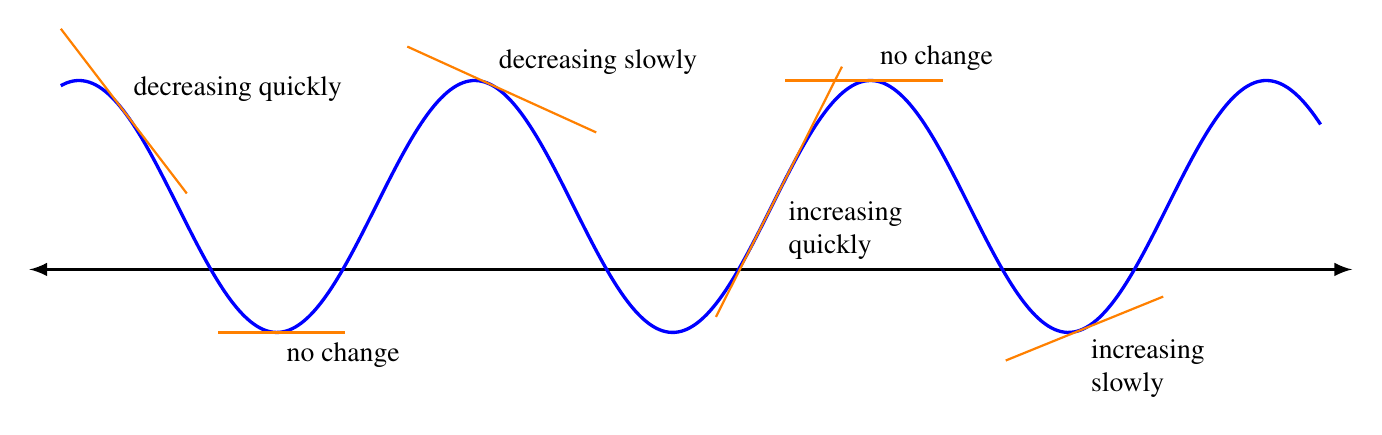
\begin{tikzpicture}[scale=0.8]
  \draw[latex-latex, very thick] (-5.5,0)--(15.5,0);

  \draw[domain=-5:15,samples=200,smooth,variable=\x, blue, very thick] plot ({\x},{1+2*sin(\x r)});
 
  \draw[domain=-5:-3,smooth,variable=\x, orange, thick] plot ({\x},{2*\x*cos(4 r) + 1 - 2*sin(4 r) + 8*cos(4 r)});
  \node[above right] at (-4,{1+2*sin(-4 r)}) {decreasing quickly};
 
  \draw[domain=-2.5:-.5,smooth,variable=\x, orange, thick] plot ({\x},{1+2*sin(-1.57 r)});
  \node[below right] at (-1.57,{1+2*sin(-1.57 r)}) {no change};
 
  \draw[domain=0.5:3.5,smooth,variable=\x, orange, thick] plot ({\x},{3.76562-0.4544*\x});
  \node[above right] at (1.8,{1+2*sin(1.8 r)}) {decreasing slowly};
 
  \draw[domain=5.4:7.4,smooth,variable=\x, orange, thick] plot ({\x},{1.98637*\x - 11.4797});
  \node[below right,text width=2cm] at (6.4,{1+2*sin(6.4 r)}) {increasing quickly};
 
  \draw[domain=6.5:9,smooth,variable=\x, orange, thick] plot ({\x},{1+2*sin(7.85 r)});
  \node[above right] at (7.85,{1+2*sin(7.85 r)}) {no change};
 
  \draw[domain=10:12.5,smooth,variable=\x, orange, thick] plot ({\x},{0.40601*\x - 5.50566});
  \node[below right,text width=2cm] at (11.2,{1+2*sin(11.2 r)}) {increasing slowly};
\end{tikzpicture}


% % HORIZONTAL spring - axis, compressed
% \begin{tikzpicture}
%   \def\H{1.1} % wall height
%   \def\T{0.3} % wall thickness
%   \def\W{3.9} % ground length
%   \def\D{0.2} % ground depth
%   \def\h{0.7} % mass height
%   \def\w{0.8} % mass width
%   \def\x{2.0} % mass x position
%   \def\dx{0.9} % extension
%   \def\y{1.22*\H} % x axis y position
%   \def\F{0.8} % force
  
%   % AXIS
%   \draw[mydashed] (\x,0) --++ (0,\y) (\x-\dx,0) --++ (0,1.1*\y);
%   \draw[axis] (\x-0.4*\W,\y) -- (\x+0.4*\W,\y) node[right] {$x$};
%   \tick{\x,\y}{-90} node[scale=0.8,above=-1] {$0$};
%   \draw[ell] (0,1.3*\h) --++ (\x,0) node[pos=0.4,fill=white,inner sep=0] {$\ell_0$};
%   \draw[dx] (\x,1.6*\h) --++ (-\dx,0)
%     node[pos=0.45,fill=white,inner sep=0,scale=0.9] {$x$};
  
%   % SPRING & MASS
%   \draw[spring,segment length=2.9] (0,\h/2) --++ (\x-\dx,0);
%   \draw[ground] (0,0) |-++ (-\T,\H) |-++ (\T+\W,-\H-\D) -- (\W,0) -- cycle;
%   \draw (0,\H) -- (0,0) -- (\W,0);
%   \draw[mass] (\x-\dx,0) rectangle++ (\w,\h) node[midway] {$m$};
%   \draw[force] (\x-\dx+0.8*\w,0.8*\h) --++ (\F,0) node[below=0,right=-1] {$\vb{F}$};
  
% \end{tikzpicture}


% % VERTICAL spring
% \begin{tikzpicture}
%   \def\H{0.25} % ceiling height
%   \def\W{1.0}  % ceiling width
%   \def\h{0.7}  % mass height
%   \def\w{0.6}  % mass width
%   \def\y{1.6}  % mass width
%   \draw[spring] (0,0) -- (0,-\y);
%   \draw[ground] (-\W/2,0) rectangle++ (\W,\H);
%   \draw (-\W/2,0) --++ (\W,0);
%   \draw[mass] (-\w/2,-\y) rectangle++ (\w,-\h) node[midway] {$m$};
% \end{tikzpicture}


% % VERTICAL spring - no mass
% \begin{tikzpicture}
%   \def\H{0.25} % ceiling height
%   \def\W{1.0}  % ceiling width
%   \def\h{0.7}  % mass height
%   \def\w{0.6}  % mass width
%   \def\y{1.6}  % mass width
%   \draw[spring] (0,0) -- (0,-\y);
%   \draw[ground] (-\W/2,0) rectangle++ (\W,\H);
%   \draw (-\W/2,0) --++ (\W,0);
%   \draw[ell] (-0.4*\W,0) --++ (0,-\y) node[midway,fill=white,inner sep=0] {$\ell_0$};
% \end{tikzpicture}


% % VERTICAL spring - extension at rest
% \begin{tikzpicture}
%   \def\H{0.25} % ceiling height
%   \def\W{1.0}  % ceiling width
%   \def\h{0.7}  % mass height
%   \def\w{0.6}  % mass width
%   \def\y{2.1}  % mass width
%   \def\F{0.8}  % force magnitude
%   \draw[spring,segment length=7] (0,0) -- (0,-\y);
%   \draw[ground] (-\W/2,0) rectangle++ (\W,\H);
%   \draw (-\W/2,0) --++ (\W,0);
%   \draw[mass] (-\w/2,-\y) rectangle++ (\w,-\h) node[midway] {$m$};
%   \draw[force] (0.4*\w,-\y-0.3*\h) --++ (0,\F) node[below right=0] {$\vb{F}$}; %=-k\Delta\ell\vu{y}
%   \draw[force] (0.3*\w,-\y-0.7*\h) --++ (0,-\F) node[above right=0] {$m\vb{g}$}; %=mg\vu{y}
%   \draw[ell] (-0.4*\W,0) --++ (0,-0.75*\y) node[midway,fill=white,inner sep=0] {$\ell_0$};
%   \draw[ell] (-0.4*\W,-0.75*\y) --++ (0,-0.25*\y) node[midway,left=0] {$\Delta\ell$};
% \end{tikzpicture}


% % VERTICAL spring - extension
% \begin{tikzpicture}
%   \def\H{0.25}     % ceiling height
%   \def\W{2.6}      % ceiling width
%   \def\h{0.7}      % mass height
%   \def\w{0.6}      % mass width
%   \def\l{0.5*\y}   % rest length without weight
%   \def\dl{0.7*\y}  % rest length with weight
%   \def\y{2.4}      % mass y position
%   \def\xy{0.38*\W} % mass y position
%   \def\F{0.8}      % force magnitude
%   \draw[spring,segment length=7.2] (0,0) -- (0,-\y);
%   \draw[ground] (-\W/2,0) rectangle++ (\W,\H);
%   \draw (-\W/2,0) --++ (\W,0);
%   \draw[axis] (-\xy,0) --++ (0,-\y-0.7*\h) node[left] {$y$};
%   \draw[axis] ( \xy,0) --++ (0,-\y-0.7*\h) node[right] {$y'$};
%   \draw[mydashed] (-\xy,-\l) --++ (2.3*\xy,0);
%   \draw[mydashed] (-\xy,-\dl) --++ (2*\xy,0);
%   \draw[mydashed] (-0.46*\W,-\y) --++ (0.92*\W,0);
%   \tick{-\xy,-\l}{0} node[left] {$0$};
%   \tick{-\xy,-\dl}{0} node[left] {$y_0$};
%   \tick{ \xy,-\dl}{180} node[right] {$0$};
%   \draw[mass] (-\w/2,-\y) rectangle++ (\w,-\h) node[midway] {$m$};
%   \draw[force] (0.4*\w,-\y-0.3*\h) --++ (0,1.6*\F) node[pos=0.9,right=0] {$\vb{F}$};
%   \draw[force] (0.3*\w,-\y-0.7*\h) --++ (0,-\F) node[above right=0] {$m\vb{g}$};
%   \draw[ell] (0.45*\W,0) --++ (0,-\l) node[midway,right=-2] {$\ell_0$};
%   %\draw[ell] (-0.4*\W,-0.75*\y) --++ (0,-0.25*\y) node[midway,left=1] {$y_0$};
% \end{tikzpicture}


% % HORIZONTAL doubly extended spring (rest position)
% \begin{tikzpicture}
%   \def\H{1.2}      % wall height
%   \def\T{0.3}      % wall thickness
%   \def\W{4.2}      % ground length
%   \def\D{0.25}     % ground depth
%   \def\h{0.6}      % mass height
%   \def\w{0.75}     % mass width
%   \def\x{1.85}     % mass x position
%   \def\lz{1.25}    % rest length (ell_0)
%   \def\ly{0.87*\H} % ell_0 y position
%   \def\y{1.19*\H}  % x axis y position
  
%   % AXIS
%   \draw[mydashed] (\x,0) --++ (0,1.14*\y) (\x+\w,0) --++ (0,1.14*\y);
%   \draw[axis] (0.15*\W,\y) --++ (0.7*\W,0) node[right=-2] {$x$};
%   \tick{\x+\w/2,\y}{-90} node[scale=0.8,above=-1] {$0$};
%   \draw[ell] (0,\ly) --++ (\lz,0) node[midway,fill=white,inner sep=0] {$\ell_0$};
%   \draw[ell] (\W,\ly) --++ (-\lz,0) node[midway,fill=white,inner sep=0] {$\ell_0$};
%   \draw[dx] (\lz,1.04*\ly) --++ (\x-\lz,0) node[pos=0.45,above=-2] {$x_1$};
%   \draw[dx] (\W-\lz,1.04*\ly) --++ (\lz+\x+\w-\W,0) node[pos=0.4,above=-2] {$x_2$};
  
%   % SPRINGS & MASS
%   \draw[spring,segment length=6] (0,\h/2) --++ (\x,0) node[pos=0.3,above=3] {$k_1$};
%   \draw[spring,segment length=6] (\W,\h/2) --++ (\x+\w-\W,0) node[pos=0.3,above=3] {$k_2$};
%   \draw[ground] (0,0) |-++ (-\T,\H) |-++ (2*\T+\W,-\H-\D) |-++
%                 (-\T,\H+\D) --++ (0,-\H) -- cycle;
%   \draw (0,\H) -- (0,0) -- (\W,0) --++ (0,\H);
%   \draw[mass] (\x,0) rectangle++ (\w,\h) node[midway] {$m$};
%   \draw[force] (\x+0.1*\w,0.9*\h) --++ (-0.2*\W,0) node[pos=0.65,above=-1] {\contour{white}{$-k_1x_1$}};
%   \draw[force] (\x+0.9*\w,0.9*\h) --++ ( 0.2*\W,0) node[pos=0.40,above=-1] {\contour{white}{$-k_2x_2$}};
  
% \end{tikzpicture}


% % HORIZONTAL doubly compressed spring (rest position)
% \begin{tikzpicture}
%   \def\H{1.2}      % wall height
%   \def\T{0.3}      % wall thickness
%   \def\W{4.2}      % ground length
%   \def\D{0.25}     % ground depth
%   \def\h{0.6}      % mass height
%   \def\w{0.85}     % mass width
%   \def\x{1.62}     % mass x position
%   \def\lz{2.03}    % rest length (ell_0)
%   \def\ly{0.87*\H} % ell_0 y position
%   \def\y{1.19*\H}  % x axis y position
  
%   % AXIS
%   \draw[mydashed] (\x,0) --++ (0,1.14*\y) (\x+\w,0) --++ (0,1.14*\y);
%   \draw[axis] (0.15*\W,\y) --++ (0.7*\W,0) node[right=-2] {$x$};
%   \tick{\x+\w/2,\y}{-90} node[scale=0.8,above=-1] {$0$};
%   \draw[ell] (0,\ly) --++ (\lz,0) node[pos=0.45,fill=white,inner sep=0] {$\ell_0$};
%   \draw[ell] (\W,\ly) --++ (-\lz,0) node[pos=0.45,fill=white,inner sep=0] {$\ell_0$};
%   \draw[dx] (\lz,1.06*\ly) --++ (\x-\lz,0) node[pos=0.4,above=-2] {$x_1$};
%   \draw[dx] (\W-\lz,1.06*\ly) --++ (\lz+\x+\w-\W,0) node[pos=0.7,above=-2] {\contour{white}{$x_2$}};
  
%   % SPRINGS & MASS
%   \draw[spring,segment length=2.9] (0,\h/2) --++ (\x,0) node[pos=0.42,above=3] {$k_1$};
%   \draw[spring,segment length=2.9] (\W,\h/2) --++ (\x+\w-\W,0) node[pos=0.35,above=3] {$k_2$};
%   \draw[ground] (0,0) |-++ (-\T,\H) |-++ (2*\T+\W,-\H-\D) |-++
%                 (-\T,\H+\D) --++ (0,-\H) -- cycle;
%   \draw (0,\H) -- (0,0) -- (\W,0) --++ (0,\H);
%   \draw[mass] (\x,0) rectangle++ (\w,\h) node[midway] {$m$};
%   \draw[force] (\x+0.65*\w,0.9*\h) --++ ( 0.2*\W,0) node[pos=0.55,above=-1] {\contour{white}{$-k_1x_1$}};
%   \draw[force] (\x+0.35*\w,0.9*\h) --++ (-0.2*\W,0) node[pos=0.60,above=-1] {\contour{white}{$-k_2x_2$}};
%   %\draw[force] (\x+0.7*\w,0.1*\h) --++ (-0.2*\W,0) node[pos=0.5,below=0] {\contour{white}{$-k_2x_2$}};
  
% \end{tikzpicture}


% % HORIZONTAL double spring
% \begin{tikzpicture}
%   \def\H{0.8}  % wall height
%   \def\T{0.3}  % wall thickness
%   \def\W{4.2}  % ground length
%   \def\D{0.25} % ground depth
%   \def\h{0.6}  % mass height
%   \def\w{0.8}  % mass width
%   \def\x{2.2}  % mass x position
%   \draw[spring,segment length=7.0] (0,\h/2) --++ (\x,0) node[midway,above=4] {$k_1$};
%   \draw[spring,segment length=2.9] (\W,\h/2) --++ (\x+\w-\W,0) node[midway,above=4] {$k_2$};
%   \draw[ground] (0,0) |-++ (-\T,\H) |-++ (2*\T+\W,-\H-\D) |-++
%                 (-\T,\H+\D) --++ (0,-\H) -- cycle;
%   \draw (0,\H) -- (0,0) -- (\W,0) --++ (0,\H);
%   \draw[mass] (\x,0) rectangle++ (\w,\h) node[midway] {$m$};
%   %\draw[force] (\x+0.1*\w,0.9*\h) --++ (-0.4*\W,0) node[midway,above=0] {$-k_1\vb{x}$};
%   %\draw[force] (\x+0.9*\w,0.9*\h) --++ ( 0.2*\W,0) node[midway,above=0] {$-k_2\vb{x}$};
% \end{tikzpicture}


% % HORIZONTAL double spring - lengths
% \begin{tikzpicture}
%   \def\H{1.2}      % wall height
%   \def\T{0.3}      % wall thickness
%   \def\W{4.2}      % ground length
%   \def\D{0.25}     % ground depth
%   \def\h{0.6}      % mass height
%   \def\w{0.8}      % mass width
%   \def\x{2.2}      % mass x position
%   \pgfmathsetmacro\dx{\x+(\w-\W)/2} % extension
%   \pgfmathsetmacro\lz{\x-\dx} % rest length (ell_0)
%   \def\ly{0.87*\H} % ell_0 y position
%   \def\y{1.19*\H}  % x axis y position
  
%   % AXIS
%   \draw[mydashed] (\x,0) --++ (0,1.14*\y) (\x+\w,0) --++ (0,1.14*\y);
%   \draw[axis] (0.15*\W,\y) --++ (0.7*\W,0) node[right=-2] {$x$};
%   \tick{\lz+\w/2,\y}{-90} node[scale=0.8,above=-1] {$0$};
%   \draw[ell] (0,\ly) --++ (\lz,0) node[midway,fill=white,inner sep=0] {$\ell_0$};
%   \draw[ell] (\W,\ly) --++ (\lz+\w-\W,0) node[pos=0.45,fill=white,inner sep=0] {$\ell_0$};
%   \draw[dx] (\lz,1.06*\ly) --++ (\dx,0) node[pos=0.45,above=-2] {$x$};
%   \draw[dx] (\lz+\w,1.06*\ly) --++ (\dx,0) node[pos=0.45,above=-2] {$x$};
  
%   % SPRINGS & MASS
%   \draw[spring,segment length=7.0] (0,\h/2) --++ (\x,0) node[pos=0.42,above=3] {$k_1$};
%   \draw[spring,segment length=2.9] (\W,\h/2) --++ (\x+\w-\W,0) node[pos=0.5,above=3] {$k_2$};
%   \draw[ground] (0,0) |-++ (-\T,\H) |-++ (2*\T+\W,-\H-\D) |-++
%                 (-\T,\H+\D) --++ (0,-\H) -- cycle;
%   \draw (0,\H) -- (0,0) -- (\W,0) --++ (0,\H);
%   \draw[mass] (\x,0) rectangle++ (\w,\h) node[midway] {$m$};
%   \draw[force] (\x+0.07*\w,0.9*\h) --++ (-0.15*\W,0) node[left=0,above=-1] {\contour{white}{$-k_1x$}};
%   \draw[force] (\x+0.93*\w,0.9*\h) --++ (-0.15*\W,0) node[pos=0.47,above=-1] {\contour{white}{$-k_2x$}};
  
% \end{tikzpicture}


\end{document}